\chapter{Proactive Policy Inference}\label{chapt:proactive_inference}

In the experiments in previous sections, an autonomous agent eventually infers a reasonable estimate of an uncontrollable agent's policy. By approximating the uncontrollable agent's $Q$-function as a linear combination of fixed and mobile features, the autonomous agent can eventually learn the hidden parameters in the transition model of a \ac{HiPMDP}, where the hidden parameter is the policy of the uncontrollable agent.

The successes in previous chapters have ignored a realistic constraint. Often, sampling a system is expensive, costing both time and wear-and-tear on mechatronic systems. This chapter will cover how an autonomous agnet can adjust its policy to improve sample efficiency.

\section{Proactive Inference}

Assuming that \agent{1} has received some initial data $D^{(1)}$, the estimated policy of the uncontrollable agent
can be improved from some initial guess $\estimate{\policy{}}_2^{(0)}$ to form $\estimate{\policy{}}_2^{(1)}$. Let's
assume that $D^{(1)}$ was incomplete, it did not contain enough data for the following algorithm to meet the
tolerance required by Assumption \ref{assump:opt_policy_err}. Therefore, \agent{1} will need to gather more data,
sets of trajectories, $D^{(b)},\ b=1,\ldots,B$. Like the \DAGGER algorithm \cite{ross2011reduction}, whenever a new dataset $D^{(b)}$ is received, the data used for inference is updated as $D\leftarrow D\cup D^{(b)}$. Ideally, $D^{(b)}$ will contain data that were lacking in all previous
batches, because, when there are not enough data, some estimates parameter elements, $\estimate{\theta}_\paramIdx$, will be
incorrect.

How can \agent{1} glean more informative data? To achieve proactive policy inference, \agent{1} needs to recognize
what parts of \policy{2} it thinks are known and unknown. Explicitly, after observing $D^{(b)}$, \agent{1} still
might have very little knowledge about $\policy{2}(x)$ -- perhaps $s_2=x$ has not yet been visited. This section
will discuss how to distinguish known and unknown policy parameters, and how \agent{1} can proactively influence the
observed data, $D$.

\begin{remark}
	The parameter vector inferred from any batch will be written $\estimate{\paramVec}^{(b)}$, which is not to
	be confused with the sampled $\paramVec^{(i)}$ in Eq. \ref{eq:gradLogLike}.
\end{remark}


\subsection{Characterizing Unknown Parameters}\label{sec:unknown_params}
By Eq. \ref{eq:true_state_trans_prob}, the transition function is determined by the policies of both agents,
\[
P((s_1',s_2')|(s_1,s_2),(a_1,a_2)) = T(s_1'|s_1,a_1) \policy{2}(a_2|(s_1,s_2))\policy{1}(a_1|(s_1,s_2)).
\]
Since we've made Assumption \ref{assump:stationary_markov} that \policy{2} is a stationary Markov policy, learning
$\policy{2}$ is equivalent to learning the dynamics of the MDP. Both problems have the same sample complexity, they
are polynomial in the size of the joint state space and the action space of the \agent{2}. With the Gaussian policy
approximation from Section \ref{sec:gauss_policy}, if the number of parameters, $W$ is much less than $|S|\times A$,
then sample complexity will be significantly reduced.

\begin{definition}
	Given two parameters $\epsilon, \varphi \in (0,1)$, a parameter $\theta_{\paramIdx}$ is $(\epsilon,
	\varphi)$-known if, with probability $1-\varphi$, the probability of the true value for $\paramElem$ is
	$\epsilon$ close to the mean of the Gaussian distribution $\normal{\mu_{\paramIdx}, \nu_{\paramIdx}}$, \ie,
	\[
	P(\abs{\paramElem - \mu_{\paramIdx}} \ge \epsilon) \le \varphi.
	\]
\end{definition}

If the estimated unknown policy parameter $\estimate{\paramSym}_w$ is $\epsilon$-close to the true (unknown) mean
$\mu_{\paramIdx}$ with probability $1-\varphi$, then we could claim  that enough knowledge has been obtained for
$\paramElem$ and treat it as a \emph{known} policy parameter. This claim is based on the Chernoff bound
\cite{kobayashi2011probability}.

Let $\Theta_\known$ be the set of known policy parameters and $\Theta_{\unknown}$ be the remaining unknown
parameters.  Next, we present a method to determine whether a state is unknown from the knowledge of these sub-sets
of $\Theta$.

First, given that each sampled parameter vector in Eq. \ref{eq:gradLogLike}, $\paramVec^{(i)}$, is a Gaussian
variable, the $\estimate{Q}$-function is distributed as a multi-variate normal:
\[
\estimate{Q}(s,a ;\paramVec^{(i)}) \sim \sum_{w=1}^W \featElem(s,a_2) \normal{\mu_w, \nu_w^2},
\]
The features, $\featElem(s,a_2),\ w=1,\ldots, W$ can be viewed as the mixing parameters.

A state $s$ is known if and only if for any $a_2 \in A$, $Q(s,a_2)$ is known. Since the $Q$-value is a mixture of
Gaussians, we'll use the mean and variance of $Q(s,a;\estimate{\paramVec}^{(b)})$ returned from Eq.
\ref{eq:gradient_update} to determine the distribution of a random variable -- the estimate of $\policy{2}(a|s)$.

If we were trying to solve a Probably-Approximatly-Correct- (PAC)-MDP \cite{Fu-RSS-14}, we would require an accuracy
in learning the transition function. For example, if the model error $\bar T(s'|s,a_1) - T(s'|s,a_1) \le
\varepsilon$ with probability $1-\varphi$, where $\bar T$ is the estimated transition function and $T$ is the true
transition function -- then the model is considered to be correct.

Based on the needed accuracy and the relation between $T$ and $\policy{2}$,
\[
P(s'|s,a_1) = T(s'|s,(a_1,a_2))\pi_2(a_2|s),
\]
we can show:
\begin{align*}
\bar P(s'|s,a_1)  -P(s'|s,a_1)
& = T(s'|s,(a_1,a_2))\left( \pi_2(a_2|s) - \bar \pi_2(a_2|s;\paramVec^{(b)})
\right)\\
& \approx T(s'|s,(a_1,a_2)) \\
& \quad \cdot \Big(\exp(Q(s,a_2)-V(s)/\kappa) \\
& \qquad\ - \exp(Q(s,a_2;\paramVec^{(b)})-V(s;\paramVec^{(b)})/\kappa) \Big)
\end{align*}

Since $Q(s,a_2;\paramVec)$ is a Gaussian, $\exp Q(s,a_2;\paramVec)$ is log-normal. Remember that to the first two
moments, the sum of lognormal random variables can be approximated by a lognormal random variable
\cite{fenton1960sum}.  The approximated value function is the log-summation of log-normal random variables: ${V
	=\kappa \log \sum \exp Q(s,a;\paramVec)/\kappa}$. This can be approximated as a Gaussian. Therefore, we can quantify
the bounded error between the estimated transition and true transition model, $\pi_2(a_2|s) - \bar
\pi_2(a_2|s;\paramVec^{(b)})$,  by directly analyzing the distribution of the log-normal random variable\\
{\(\exp(Q(s,a_2;\paramVec^{(b)})-V(s;\paramVec^{(b)}))\)}.

We will use the linear combination of parameter-variances to quantify the variance of the Q-function.
\begin{equation}\label{eq:state_action_uncertainty}
\Omega(s,a_2)=\sum_{w=1 \in \Theta_{\unknown}} \nu_w^2 \phi_w^2(s,a_2).
\end{equation}
This can now be used as a metric for \agent{1} to either query, or explore, for the most informative data-batch
$D^{(b)}$. We'll use a threshold to determine the assignment of parameters into the known and unknown parameter sets.
\begin{equation*}
	\paramElem \in \begin{cases}
					\Theta_{\known} & \text{if}\ \nu_w \leq \vartheta \\
					\Theta_{\unknown} & \text{Otherwise} \\
					\end{cases}
\end{equation*}

%\todo[inline]{If the random variable $\pi_2$ is \emph{log}-normal, shouldn't I be using the variance of the
%	log-normal distribution to reason about weather a state is known or not?
%	\[
%	X(s,a_2) = \left[\exp(\Omega(s,a_2) - 1)\right] \exp(2 Q(s,a_2) + \Omega(s,a_2)^2)
%	\]
%	I have been using Eq. \ref{eq:state_action_uncertainty} to guide the experiments.... }

\section{Single Agent Proactive Inference}
In a scenario where \agent{1} simply watches \agent{2} but sample efficiency is still a concern, assume that \agent{1} can request \agent{2} to give a demonstration that starts from a state that has a high value of $\Omega(s,a_2)$. However, \agent{1} cannot directly request \agent{1} to start at state $s$ and take $a_2$ because that might violate the policy of \agent{2}.

Instead, after new data is observed $D^{(b)}$, we'll allow agent one to set the initial state-distribution of \agent{2}, $I_0$. The initial state distribution will be proportional to the total state uncertainty:
\begin{equation}\label{eq:active_initial_set}
I_0^{(b)} = \frac{\sum_{a_2} \Omega(s,a_2)}{\sum_s \sum_{a_2} \Omega(s,a_2)}
\end{equation}

\begin{figure}[htb]
	\begin{center}
		\fbox{
			\begin{minipage}{0.6\textwidth}
				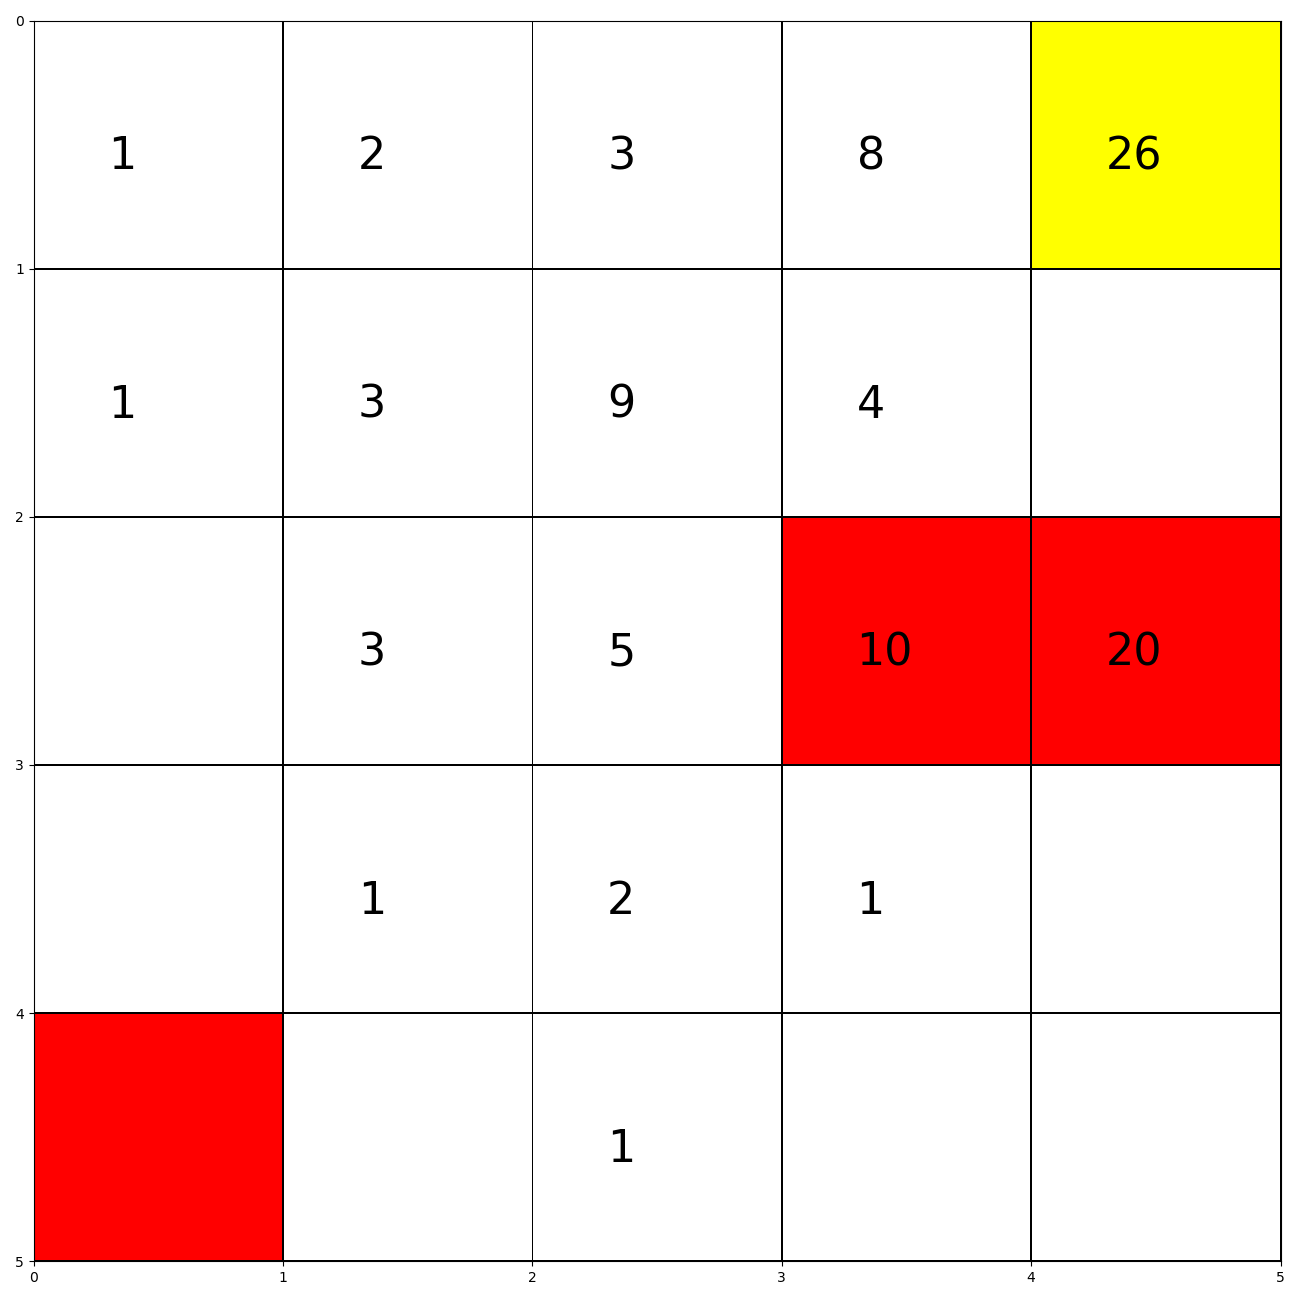
\includegraphics[width=\textwidth]{single_agent_minimal_demo}
				\caption{A set of rollouts of $\policy{2}$ that contains very few state-action samples.}
				\label{fig:single_agent_minimal_demo}
			\end{minipage}
		}
	\end{center}
\end{figure}
Given a minimal demonstration, Fig. \ref{fig:single_agent_minimal_demo}, the initial state distribution that \agent{1} would request $s_2^{(0)}$ be drawn from looks like Fig. \ref{fig:single_agent_uncertainty_surface}. Note that in this figure, the highest uncertainty is the cell $24$, the $\emph{South-East}$ (lower-left) corner.

\begin{figure}[htb]
	\begin{center}
		\fbox{
			\begin{minipage}{0.6\textwidth}
				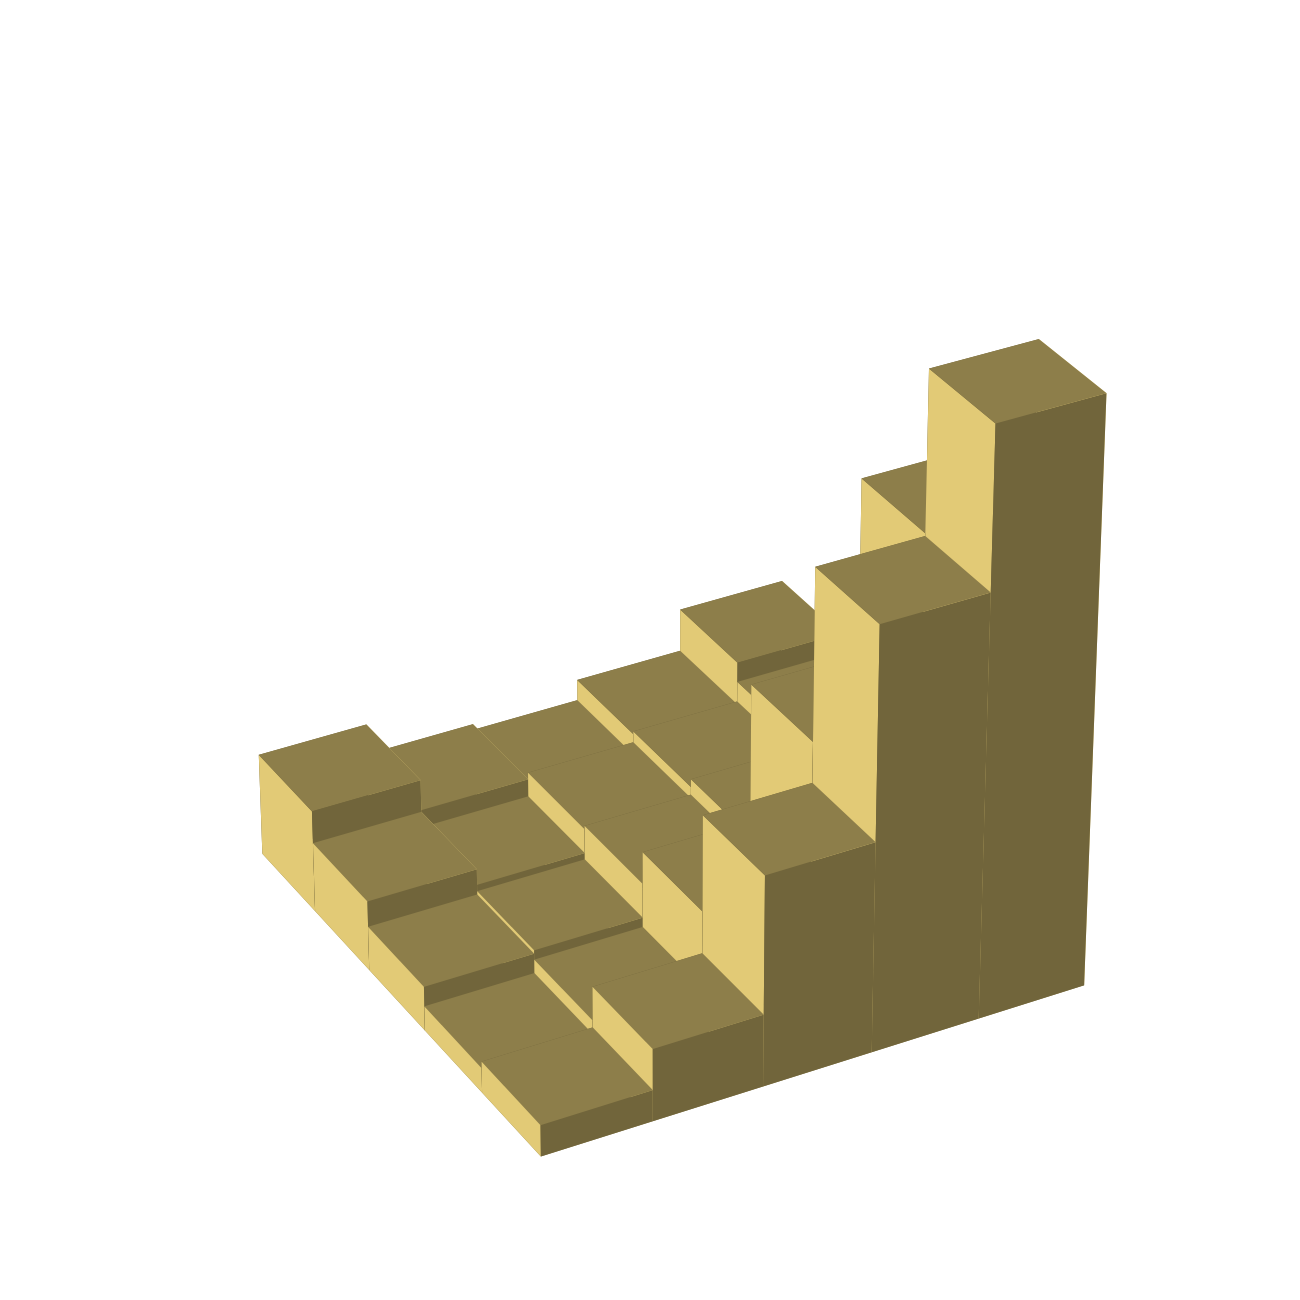
\includegraphics[width=\textwidth]{single_agent_uncertainty_surface}
				\caption{$P(s_2^{(0)}) \sim I_0$ as defined by Eq. \ref{eq:active_initial_set}}
				\label{fig:single_agent_uncertainty_surface}
			\end{minipage}
		}
	\end{center}
\end{figure}

The algorithm for proactive inference in the single agent case, Alg. \ref{alg:single_agent_batch}, requires the user to determine if $\mathsf{do\_active\_update}$ is set to $\mathsf{True}$ or $\mathsf{False}$. If $\mathsf{do\_active\_update}=\mathsf{True}$ then the initial distribution for the trajectories is set proportional to the policy uncertainty in Eq. \ref{eq:active_initial_set}. Otherwise, $s_2^{(0)} \sim \mathcal{U}(0,|S|)$

Another note is that the gradient step size, $\lambda$ must now adapt as the data set size, $|D|$, grows; see Remark \ref{rem:graidient_variability}. Setting it to be inversely proportional to the nominal log-probability of the observed dataset, the constant term in Eq. \ref{eq:log_prob_demo} is often a good choice. If that constant term is zero, i.e. transitions are deterministic, the cardinality of the data-set can be used:
\begin{equation}\label{eq:adaptive_step_size}
\begin{aligned}
	\lambda & = \frac{1}{-10 \left[ \sum_{t=0}^{\abs{\tau_d}-1} \log P \left(s^{(t+1)}|(s, a_1, o_2)^{(t)}\right)\right]},\ \text{or}\\
		& = \frac{1}{10(|D|+1)}
		\end{aligned}
\end{equation}

	\begin{algorithm}
	\caption{Single agent mini-batch inference}
	\label{alg:single_agent_batch}
	\begin{algorithmic}[1]
		\State Define Inference model $Y=(S_2,A_2,T,\featFunc)$
		\State Set $\mathsf{do\_active\_update}=(\mathsf{True}|\mathsf{False})$
		\State $I_0^{(0)} = \mathcal{U}(0,|S|)$\Comment{Sample first data set uniformly.}
		\State $D=\emptyset$ \Comment{Initialze dataset to be empty}
		\State $\vect{\mu}^{(0)} = \vect{0}$, $\vect{\nu}^{(0)} = \vect{1}$ 
		\For{$b \in [1,B]$}
		
		\State $D^{(b)} \leftarrow \mathsf{Rollout}(|D|,|\traj|I_0^{(b)})$
		\State $D \leftarrow D \cup D^{(b)}$
		\State $\lambda \leftarrow $ Eq. \ref{eq:adaptive_step_size}
		\State
		$\vect{\nu}^{(b)} , \estimate{\policy{}}_2(s;\vect{\mu}^{(b)})
		\leftarrow \mathsf{Infer}(D,Y,\vect{\mu}^{(b-1)}, \vect{\nu}^{(b-1)} )$
		\Comment{Sect. \ref{sec:policy_obj}}
		\If{$\mathsf{do\_active\_update}$}
		\State $I_0^{(b)} = \mathsf{Update}(\vect{\nu}^{(b)}, \featFunc)$
		\Comment{Eq. \ref{eq:state_action_uncertainty} \& \ref{eq:active_initial_set}}
		\EndIf
		\EndFor
	\end{algorithmic}
\end{algorithm}

For simplicity, we'll define a \emph{rollout} procedure, Algorithm \ref{alg:rollout} which is equivalent to sampling a set of trajectories.

	\begin{algorithm}
	\caption{Rollout}
	\label{alg:rollout}
	\begin{algorithmic}[1]
		\Procedure{Rollout}{$|D|,|\traj|, I_0, \policy{1}, \policy{2}$}
		\State $D=\emptyset$
		\For{$d\ \in |D|$}
		\State Sample $s_2^{(t=0)}$ from $I_0$
		\State $\traj_0 = s_2^{(0)}$
		\For{$t=1\ to\ |\traj_d|$}
		\State Sample $s_2^{(t)}$ from $p(s_2^{(t)}|s_2^{(t-1)},\policy{1}, \policy{2})$
		\Comment{Eq. \ref{eq:true_state_trans_prob}}
		\State $\traj_t = s_2^{(t)}$
		\EndFor
		\State $D = D\cup \traj_d$
		\EndFor
		\State \textbf{return} $D$
		\EndProcedure
	\end{algorithmic}
\end{algorithm}


\subsection{Experimental Results}

Here, we'll show that we can accelerate the convergence of $\estimate{\policy{}}_2^{(b)}$ as we observe more batches of data $D^{(b)}$. Similar to Section \ref{sec:single_agent_experiment}, the transition function is stochastic, see the motion model in Table \ref{table:motion_model}. The true agent policy is again described by Fig. \ref{fig:single_agent_2_policy} where \agent{2} tries to avoid the red obstacles. The algorithm parameters are listed in Table \ref{table:single_agent_active_alg_params_short} and inference parameters are listed in Table \ref{table:single_agent_active_hyper_params}.

    \begin{table}[htb]
	\centering
	\begin{tabular}{c|l l}
		$B$ & $20$ & Number of batches (updates to $\estimate{\policy{}}_2$)\\
		$|D|$ & 2 & Trajectories added per batch \\
		$|\traj|$ & 4 & Trajectory length \\
	\end{tabular}
	\caption{Parameters for single-agent active inference (Alg. \ref{alg:single_agent_batch})}
	\label{table:single_agent_active_alg_params_short}
\end{table}


\begin{table}[htb]
	\centering
	\begin{tabular}{c|l l}
		$K$ & $\mathbf{7}$ & Number of kernels\\
		$\kernStdDev_{\kernIdx}$ & $2.0,\ \forall l$ & Identical kernel standard-deviations\\
		$c_{\kernIdx}$ & -- & (Kernel Centers) Same as Fig. \ref{fig:single_agent_policy_7_kernels}\\
		$\kappa$ & $0.5$ & Temperature of $\estimate{\policy{}}_2$. Eq. (\ref{eq:policy_model}) \\
		$\lambda$ & -- & See Eq. \ref{eq:adaptive_step_size} \\
		$\eta$ & $0.2$ & Gradient velocity memory\\
		$m$ & 1000 & Per iteration sample size of $\paramVec\sim \rho$\\
		$\Lambda$ & $60$ & Moving average buffer length for $\mathsf{HIST}(\logLike)$ \\
		$\zeta$ & $0.001$ & Gradient ascent termination when $\Delta\mathsf{HIST}(\logLike) < \zeta$\\
		$\mu_{0}$ & $0.0$ & Initial parameter means\\
		$\nu_{0}$ & $1.0$ & Initial parameter standard-deviations\\
		$\nu_{min}$ & $0.4$ & Minimum parameter standard-deviation\\
		$\vartheta$ & $0.4$ & Threhold for inclusion in $\Theta_{\known}$\\
	\end{tabular}
	\caption{Hyper-parameters used for multi-agent inference.}
	\label{table:single_agent_active_hyper_params}
\end{table}

If $\mathsf{do\_active\_update}=\mathsf{True}$, we'll consider that trial of Alg. \ref{alg:single_agent_batch} to be \emph{active}, otherwise, it was \emph{passive} inference. Figure \ref{fig:single_agent_active_error} shows that updating the initial distribution with Eq. \ref{eq:active_initial_set} produces faster convergence to a minimum inference error. The solid lines represent the average $\OneNorm{\policy{2},\estimate{\policy{}}_2}$ over $50$ trials.



\begin{figure}[!htb]
	\begin{center}
		\fbox{
			\begin{minipage}{0.75\textwidth}
				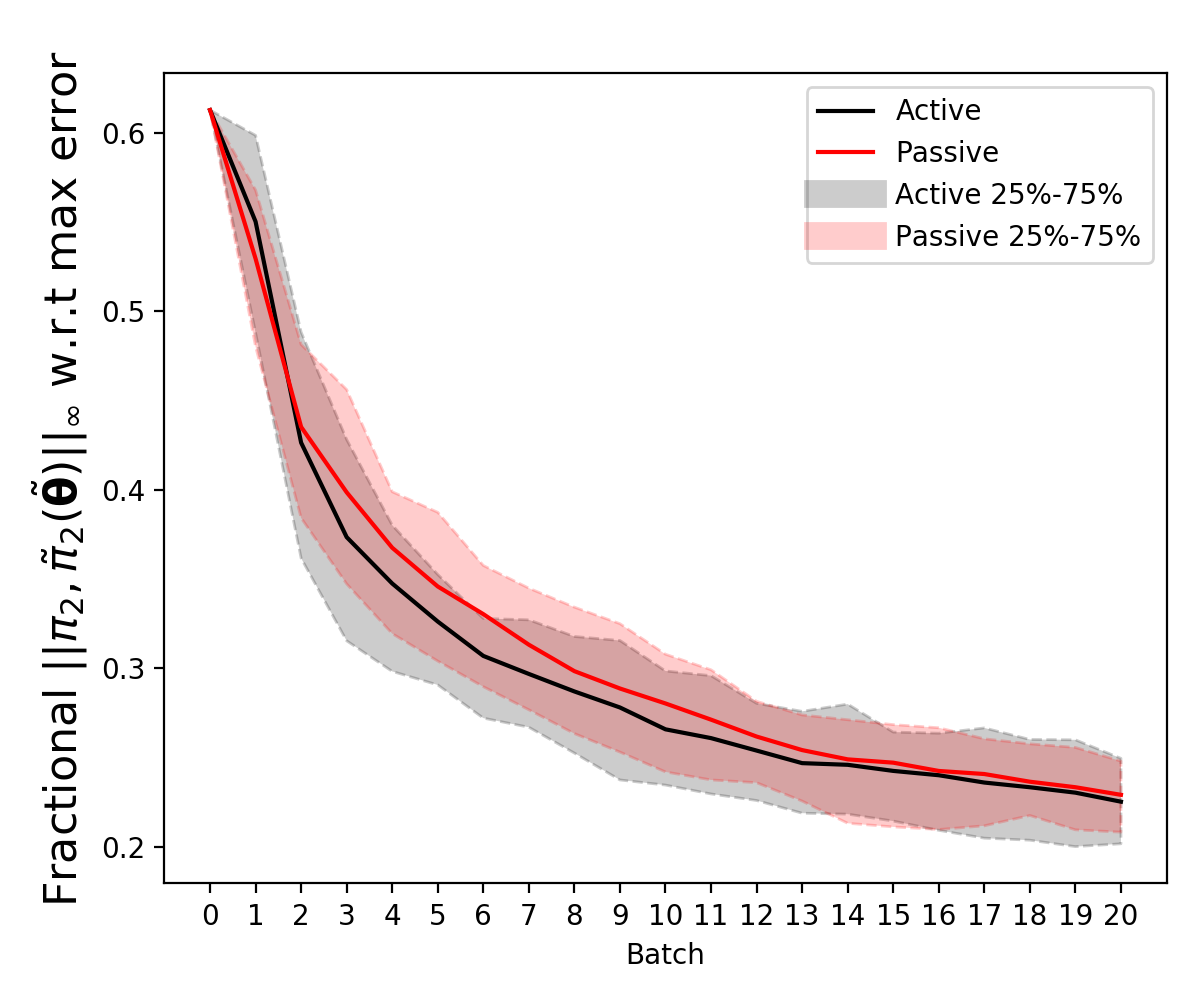
\includegraphics[width=\textwidth]{single_agent_active_inf_norm}
				\caption{50 trial average: Fraction of max $\OneNorm{\policy{2},\estimate{\policy{}}_2}$ with parameters in Table}
				\label{fig:single_agent_active_error}
			\end{minipage}
		}
	\end{center}
\end{figure}

\subsubsection{Ergodicity concerns}

In the previous experiment, the trajectories were very short and only $2$ were added to $D$ to each batch. This frugal amount of data is what allowed the \emph{active} update to $I_0$ to outperform the original uniform sampling. With the stochastic transition model in Table \ref{table:motion_model}, any trajectory of appreciable length is likely to contain several ``slips'' to an unintended grid-cell. This, essentially, increases the available information in an observed data-set. This was previously mentioned in Section \ref{sec:multi_agent_model}, we can now justify that claim.

Following Definition 1 in \cite{Hanawal2017LearningPolicies}, the fundamental matrix of the Markov chain $\mathcal{M}_{\policy{2}}$ is:
\[
Z = (T + \mathbf{1}\vect{\policy{2}}^{\intercal})^{-1},
\]
where $T$ is the transition probability matrix from Sec. \ref{sec:hipmdp}, $\mathbf{1}$ represents a vector of ones, and $\vect{\policy{2}}$ is the vector representation of the true policy of \agent{2}. Now, Definition 2 in \cite{Hanawal2017LearningPolicies} defines the \emph{ergodic coefficient} of a probability matrix (one with equal row sums) as:
\[
e(Z) = \frac{1}{2}\max_{i,j} \sum_s |z_{is} - z_{js}|.
\]
\quotationMarks{The ergodic coefficient of [$\mathcal{M}_{\policy{2}}$] indicates the sensitivity of [the] stationary distribution}\cite{Hanawal2017LearningPolicies}. 

\todo[inline]{Calculate the change in $e(Z)$ when using stochastic transition and deterministic transitions. Discuss those numbers here.}

To show this assertion, we'll rerun the single-agent \emph{active}$/$\emph{passive} experiment with more data available as stated in Table \ref{table:single_agent_active_alg_params_long}.

    \begin{table}[htb]
	\centering
	\begin{tabular}{c|l l}
		$B$ & $20$ & Number of batches (updates to $\estimate{\policy{}}_2$)\\
		$|D|$ & $\mathbf{10}$ & Trajectories added per batch \\
		$|\traj|$ & $\mathbf{6}$ & Trajectory length \\
	\end{tabular}
	\caption{Parameters for longer single-agent active inference (Alg. \ref{alg:single_agent_batch})}
	\label{table:single_agent_active_alg_params_long}
\end{table}

\begin{figure}[htb]
	\begin{center}
		\fbox{
			\begin{minipage}{0.75\textwidth}
				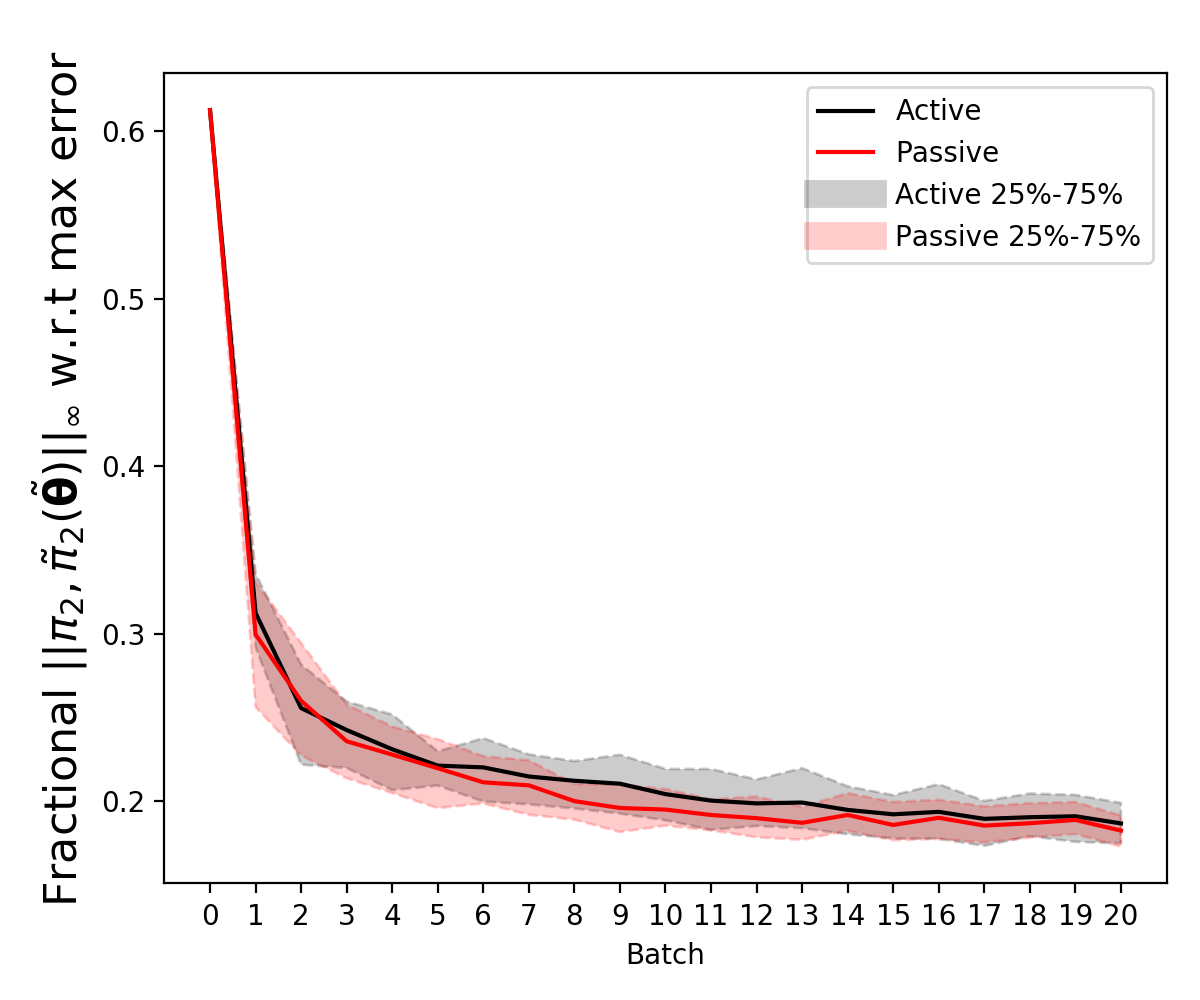
\includegraphics[width=\textwidth]{single_agent_passive_inf_norm}
				\caption{50 trial average: Fraction of max $\OneNorm{\policy{2},\estimate{\policy{}}_2}$ with Algorithm parameters in Table \ref{table:single_agent_active_alg_params_long}.}
				\label{fig:single_agent_passive_error}
			\end{minipage}
		}
	\end{center}
\end{figure}

In Figure \ref{fig:single_agent_passive_error}, we still average over $50$ trials of both \emph{active}$/$\emph{passive} flavors of Algorithm \ref{alg:single_agent_batch}. The averages of the passive trial outperform the active algorithm. Uniformly sampling 10 initial states produces variability over the trajectories added to $D$ in the $b^\text{th}$ batch and adjusting the initial distribution with Eq. \ref{eq:active_initial_set} produces less informative data in comparison.



\section{Multi-agent Proactive Inference}

Finally, we can address how \agent{1} can adjust its policy to glean the most information about \policy{2} in a dataset. This section will introduce a bonus reward used to help \agent{1} proactively explore the state-space. Like the experiments in Chapter \ref{chapt:multi_agent}, the environment has no obstacles and the transition function is deterministic.

\subsection{Asymptotic Discount Optimal Policies}\label{sec:ADO_policy}

First, we'll justify why this algorithm allow \agent{1} to solve for the its optimal policy. In Chapter 2.5 of \cite{hernandez2012adaptive}, Hern\'andez-Lerma shows that an \textit{adaptive}  \ac{MDP} will
converge to the optimal value function if the parameter estimate converges to the true parameter. Remember Assumption \ref{assump:opt_policy_err}; the true \policy{2} can be
sufficiently represented with an optimal parameter.  The author formally proves that if $\estimate{\paramVec}^{(b)}
\rightarrow \optimal{\paramVec}$ as $b \rightarrow \infty$, then $V(s;\estimate{\paramVec}^{(b)}) \rightarrow
\optimal{V}(s;\optimal{\paramVec})$. In other words, if \agent{1} can eventually infer the policy of \agent{2}, \agent{1} will then be able to plan an optimal policy to complete its task. 

\subsection{Multi-agent Algorithm}
	There are two different options for Algorithm \ref{alg:multi_agent_batch}. The \emph{passive} implementation uses $\mathsf{use\_bonus\_reward}=\mathsf{False}$, while the \emph{active} implementation uses $\mathsf{use\_bonus\_reward}=\mathsf{True}$.

	\begin{algorithm}
	\caption{Multi-agent mini-batch inference}
	\label{alg:multi_agent_batch}
	\begin{algorithmic}[1]
		\State Define \ac{HiPMDP} $\mathcal{M} = (S,A,T,\gamma,R^{o})$
		\State Define Inference model $Y=(S,A_2,T,\featFunc)$
		\State Set $\mathsf{use\_bonus\_reward}=(\mathsf{True}|\mathsf{False})$
		\State Set $I_0$
		\State $D=\emptyset$
		\State $\vect{\mu}^{(0)} = \vect{0}$, $\vect{\nu}^{(0)} = \vect{1}$ 
		\State Set $\estimate{\policy{}}_2^{(0)}(s)$ so $\mathsf{DIST}(A_2)\sim \mathcal{U}$ 
		\For{$b \in [1,B]$}
		\State $\policy{1}^{(b)} \leftarrow \mathsf{Solve}(\mathcal{M},\estimate{\policy{}}_2^{(b-1)}(s) )$
			\Comment{Use \ac{EM} from Sect. \ref{sec:EM}}
		\State $D^{(b)} \leftarrow  \mathsf{Rollout}(|D|,|\traj|I_0^{(b)},\policy{1}^{(b)}, \policy{2})$
			\Comment{Always roll out with \emph{true} \policy{2}.}
		\State $D \leftarrow D \cup D^{(b)}$
		\State $\lambda \leftarrow $ Eq. \ref{eq:adaptive_step_size}
		\State
		$\vect{\nu}^{(b)} , \estimate{\policy{}}_2(s;\vect{\mu}^{(b)})
		\leftarrow \mathsf{Infer}(D,\mathcal{M},Y,\vect{\mu}^{(b-1)}, \vect{\nu}^{(b-1)} )$
		\Comment{Sect. \ref{sec:policy_obj}}
		\If{$\mathsf{use\_bonus\_reward}$}
		\State $R(s,a_1) = R^{o}(s,a_1) \mathsf{Bonus}(\vect{\nu}^{(b)}, \featFunc)$
		\Comment{Eq. \ref{eq:state_action_uncertainty} \& \ref{eq:bonus_reward}}
		\EndIf
		\EndFor
	\end{algorithmic}
\end{algorithm}


	\subsubsection{Passive Implementation}
	 The first is if \agent{1} simply updates $\policy{1}^{(b)}$ by including the new inference  $\estimate{\policy{}}_2^{(b)}$; \agent{1} will
    simply exploit the information from $D^{(b)}$ so that $\policy{1}^{(b)}(s;\estimate{\paramVec})$ maximizes the expected discounted reward,
    as shown in Section \ref{eq:bellman_estim}. This is considered to be a \textit{passive} implementation.

	\subsubsection{Active Implementation}
     The second option is for \agent{1} to \textit{proactively} seek the most informative $D^{(b)}$.  Gathering data
     about any unknown parameter elements will be given to \agent{1} as a bonus reward; \agent{1} proactively improves
     the inference of $\estimate{\policy{}}_2$. Therefore, \agent{1} needs to determine which
     $\estimate{\theta}_\paramIdx$\!'s are unknown. This is discussed in Section \ref{sec:bonus_reward}; after each batch, a bonus reward is added to the original reward function $R^{o}$.


\subsection{Bonus Reward}\label{sec:bonus_reward}


    What we would like to do is give \agent{1} a bonus reward whenever \agent{2} takes an action for which
    $\estimate{Q}(s,a_2)$ has a large $\Omega(s,a_2)$, see Eq. \ref{eq:state_action_uncertainty}. Since \agent{1} can not actually control \agent{2} to take an
    ``uncertain" action $a_2$ at a joint state $s$, we build an exploration bonus reward at each joint state.

    Using the original reward function of the robot from Def. \ref{def:hipmdp}, the reward including an exploration
    bonus is defined as
    \[
    \hat R (s,a) = R(s,a) + \delta R(s)
    \]
    and
    \[\delta R(s)  \propto \sum_{a_2\in A}\sum_{\theta_w\in \Theta_\unknown} \nu_w^2 \phi^2_w(s,a_2)
    \]
    In practice, we can select a constant $B$ and define
    \begin{equation}\label{eq:bonus_reward}
    \delta R(s) = B \sum_{a_2\in A}\sum_{\theta_w\in \Theta_\unknown} \nu_w^2 \phi_w^2(s,a).
    \end{equation}
    The constant $B$ has a role of weighting between exploration and exploitation.

    \par
    The exploration bonus has the following property: When all parameters becomes known, the exploration bonus will
    become zero and the policy recovers to the optimal policy with respect to the original reward function. By
    definition, for the same estimate of  $\paramVec$, and for any two pairs $(x,a_1), (y,a_2),\ \forall\ x,y\in S_2 | x
    \neq y$, the uncertainty in $Q(x,a_1)$ is greater than that of $Q(y,a_2)$ if $\sum_{a_2\in A}\sum_{\theta_w\in
    \Theta_\unknown} \nu_2^2 \phi^2_w(x,a_2) > \sum_{a_2\in A}\sum_{\theta_w\in \Theta_\unknown}  \nu_w^2
    \phi^2_w(y,a_2)  $, and thus exploring any joint states $s=(s_1,x), \forall s_1 \in S_1$ will receive a higher
    exploration bonus.


\subsection{Proactive Multi-agent Experiment}

	For this experiment, we're interested in a configuration where \agent{1} and \agent{2} are essentially forced to interact. The initial state for \agent{1} will always be the \emph{South-East} (lower-left) corner, cell $24$. Its goal is to reach the \emph{North-West} (upper-left) corner, cell $0$. Similar to the multi-agent experiment in Section \ref{sec:multi_agent_inference_experiment}, \agent{2} will be trying to reach the \emph{North-East} (upper-right) corner, cell $4$. In this experiment, \agent{2} will always start in the \emph{South-West} (lower-left) corner, cell $20$. The transition model is deterministic, actions succeed with probability 1. Also, a collision results in a sink-state. The transition to a sink-state is known to \agent{1}, so it tries to avoid \agent{2} in general but the inclusion of the bonus-reward does affect that slightly.
	
	The bonus-reward coerces \agent{1} to make sub-optimal actions so that an informative joint-state is reached, \agent{2} makes informative actions, and the $\OneNorm{\policy{2},\estimate{\policy{}}_2}$ converges faster than with the passive approach; see Figure \ref{fig:multi_agent_active_error}

    \begin{table}[htb]
	\centering
	\begin{tabular}{c|l l}
		$B$ & $30$ & Number of batches (updates to $\estimate{\policy{}}_2$ and \policy{1})\\
		$|D|$ & 10 & Trajectories added per batch \\
		$|\traj|$ & 10 & Trajectory length \\
	\end{tabular}
	\caption{Parameters for multi-agent active inference (Alg. \ref{alg:multi_agent_batch})}
	\label{table:multi_agent_active_alg_params}
\end{table}


\begin{table}[htb]
	\centering
	\begin{tabular}{c|l l}
		$K$ & $\mathbf{9}$ & Number of kernels\\
		$\kernStdDev_{\kernIdx}$ & $2.0,\ \forall l$ & Identical kernel standard-deviations\\
		$c_{\kernIdx}$ & $[0:4:24]$ & Kernel Centers every $4^\text{th}$ cell (forms an ``$\mathsf{X}$'')\\
		$\kappa$ & $0.5$ & Temperature of $\estimate{\policy{}}_2$. Eq. (\ref{eq:policy_model}) \\
		$\mathbf{I_0}$ & $(20,24)$ & Constant initial state for all $\traj$'s. \\
		$\lambda$ & -- & See Eq. \ref{eq:adaptive_step_size} \\
		$\eta$ & $0.2$ & Gradient velocity memory\\
		$m$ & 1000 & Per iteration sample size of $\paramVec\sim \rho$\\
		$\Lambda$ & $60$ & Moving average buffer length for $\mathsf{HIST}(\logLike)$ \\
		$\zeta$ & $0.001$ & Gradient ascent termination when $\Delta\mathsf{HIST}(\logLike) < \zeta$\\
		$\mu_{0}$ & $0.0$ & Initial parameter means\\
		$\nu_{0}$ & $1.0$ & Initial parameter standard-deviations\\
		$\nu_{min}$ & $0.4$ & Minimum parameter standard-deviation\\
		$\vartheta$ & $\mathbf{0.8}$ & Threhold for inclusion in $\Theta_{\known}$\\
	\end{tabular}
	\caption{Hyper-parameters used for multi-agent inference.}
	\label{table:single_agent_active_hyper_params}
\end{table}

\begin{figure}[htb]
	\begin{center}
		\fbox{
			\begin{minipage}{0.75\textwidth}
				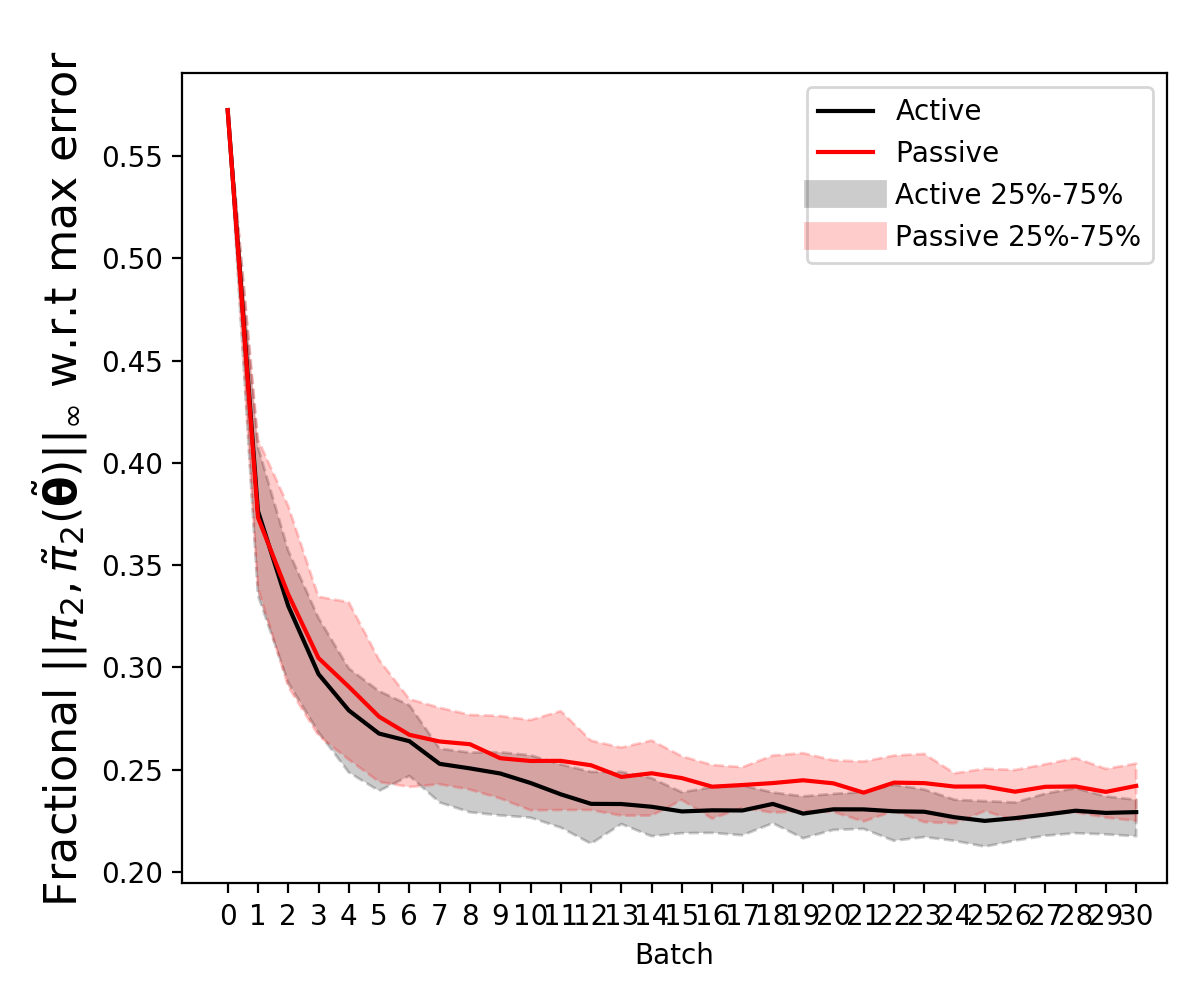
\includegraphics[width=\textwidth]{multi_agent_active_inf_norm}
				\caption{50 trial average: Fraction of max $\OneNorm{\policy{2},\estimate{\policy{}}_2}$ with Algorithm parameters in Table \ref{table:multi_agent_active_alg_params}.}
				\label{fig:multi_agent_active_error}
			\end{minipage}
		}
	\end{center}
\end{figure}


\begin{figure}[htb]
	\begin{center}
		\fbox{
			\begin{minipage}{0.75\textwidth}
				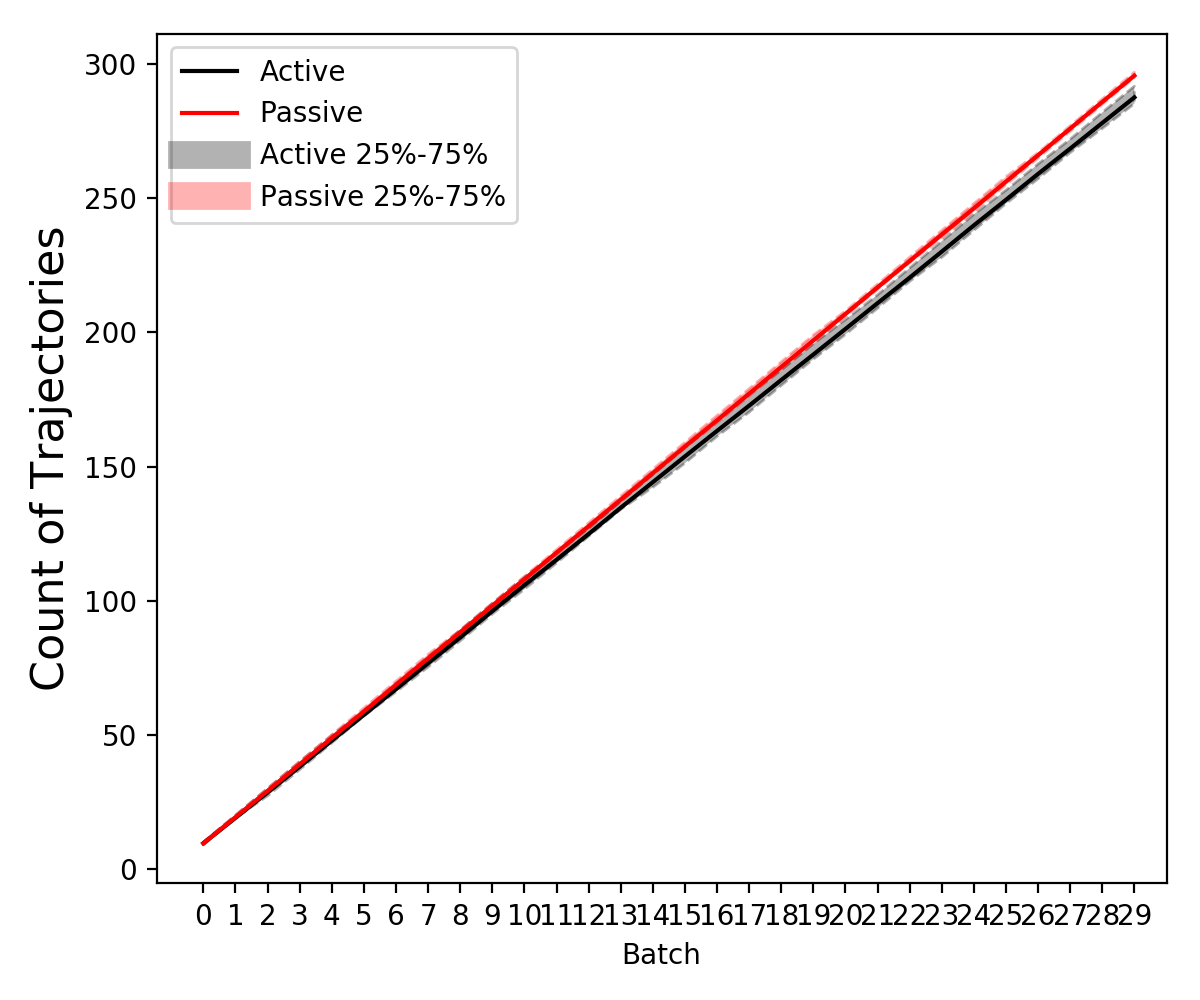
\includegraphics[width=\textwidth]{multi_agent_active_goal_count}
				\caption{50 trial average: \agent{1} reaches cell=0 (goal) with Algorithm parameters in Table \ref{table:multi_agent_active_alg_params}.}
				\label{fig:multi_agent_goal_count}
			\end{minipage}
		}
	\end{center}
\end{figure}

\subsubsection{Discussion}
\todo[inline]{Add plot of $\OneNorm{\optimal{\policy{1}}, \policy{1}^b}$ and discuss}


